\section{Результаты}
Молекула трифторметанола было оптимизирована методом B3LYP/6-31G. Было предположено, что TS является геометрия, в котором атомы O и F заслонены. После этого было оптимизировано TS.

Энергии полеченных геометрий приведены ниже: 
\begin{table}[H]
    \caption{Значения составляющих полной энергии TS и ES (в Хартри)} \label{tab:my-table}
        \begin{center}
            \begin{tabular}{|c|c|c|}
            \hline
             & ES & TS \\ \hline
            \begin{tabular}[c]{@{}c@{}}Кинетическая энергия\\ электронов\end{tabular} & 411.356 & 411.351 \\ \hline
            \begin{tabular}[c]{@{}c@{}}Потенциальная энергия\\ электронов\end{tabular} & -824.543 & -824.536 \\ \hline
            \begin{tabular}[c]{@{}c@{}}Электрон-электронное\\ взаимодействие\end{tabular} & 356.644 & 356.576 \\ \hline
            \begin{tabular}[c]{@{}c@{}}Электрон-ядерное\\ взаимодействие\end{tabular} & -1380.896 & -1380.760 \\ \hline
            \begin{tabular}[c]{@{}c@{}}Ядер-ядерное\\ взаимодействие\end{tabular} & 199.710 & 199.647 \\ \hline
            \textbf{Полная энергия} & \textbf{-413.187} & \textbf{-413.185} \\ \hline
            \end{tabular}
        \end{center}
    \end{table}

Высота потенциально барьера составляем 0.002 Хартри = 0.054 eV. 

Расчеты проводились при температуре $T = 298.15K$. Величина $\frac{\Delta E}{kT} = 2.1$. Процесс преодолим, хотя малоэффективен.

\begin{figure}[H]
\centering
\captionsetup{justification=centering}
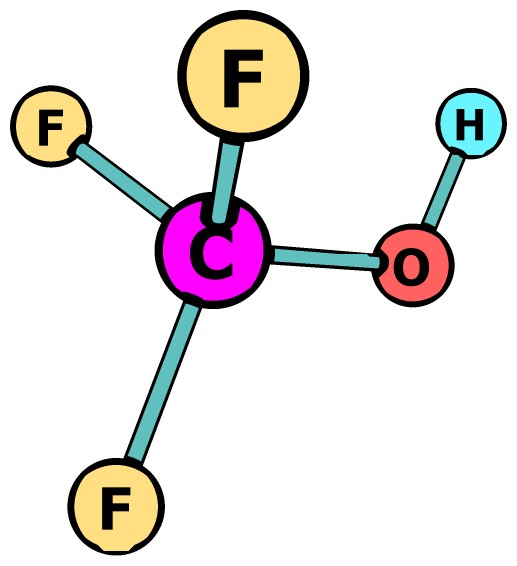
\includegraphics[scale=0.3]{fig/0.jpg}
\caption{ES молекулы трифторметанола.}
\end{figure}

\begin{figure}[H]
\centering
\captionsetup{justification=centering}
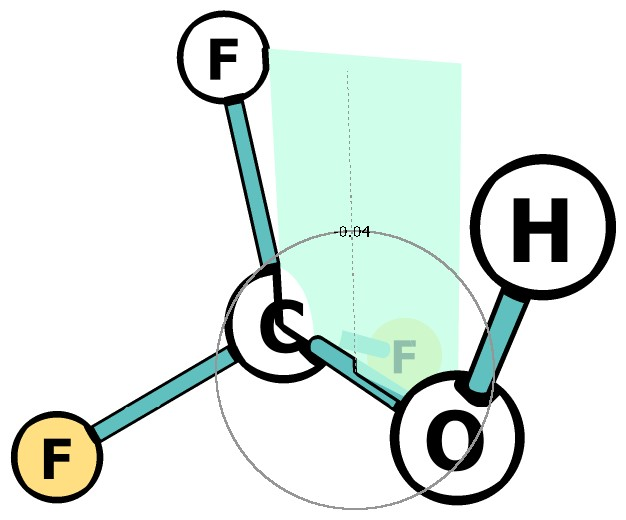
\includegraphics[scale=0.3]{fig/1.jpg}
\caption{TS молекулы трифторметанола.}
\end{figure}
